\documentclass[fontsize=12pt]{scrartcl}
\usepackage[margin=0.5in, a4paper]{geometry}
\usepackage{tikz}
\usepackage{amsmath}
\usepackage{pgfplots}
\usepackage{siunitx}
\usetikzlibrary{calc,patterns,angles,quotes}
\begin{document}
Reflect the vector in the line $y=x$:
\newline
\newline
\begin{tabular}{p{9cm}p{9cm}}
a) 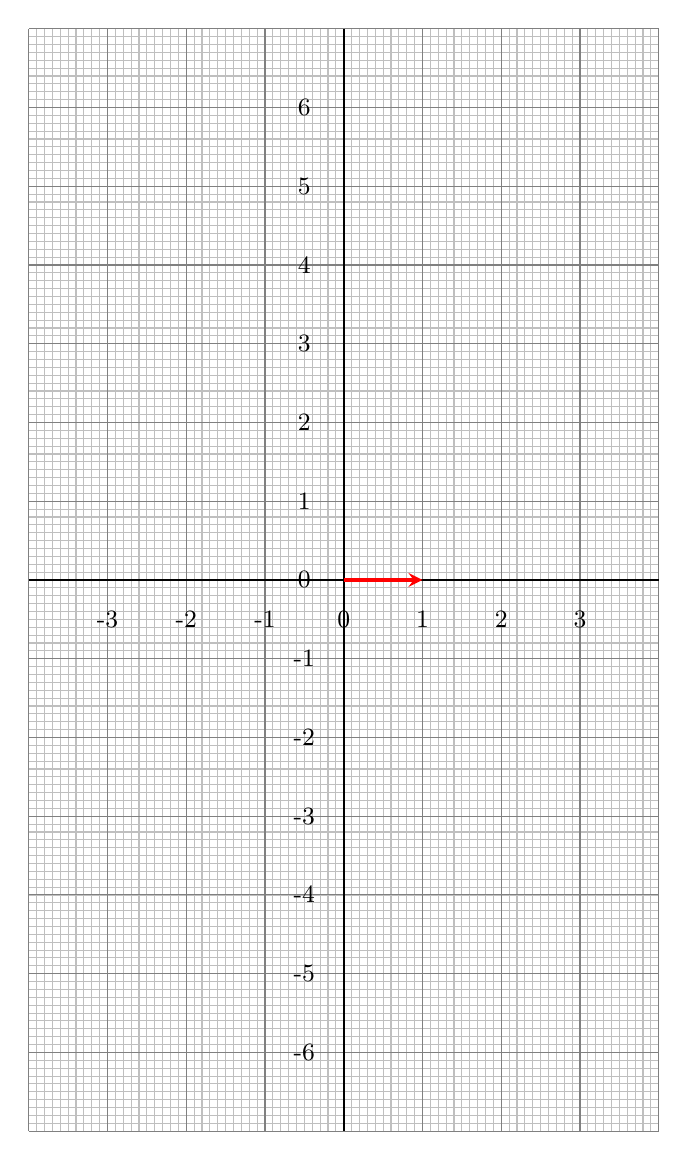
\begin{tikzpicture}
\draw[thin, step=0.1cm,color=lightgray] (-4,-7) grid (4,7);
\draw[thin, step=1cm,color=gray] (-4,-7) grid (4,7);
\draw[thick] (-4,0)--(4,0);
\draw[thick] (0,7)--(0,-7);
\foreach \x in {-3,...,3}{
  \node at (\x,-0.5)  {\small{\x}};
}
\foreach \y in {-6,...,6}{
  \node at (-0.5,\y)  {\small{\y}};
}
\draw [very thick, red, -stealth] (0,0)--(1,0);
\end{tikzpicture}
 \quad $answer$
&b) 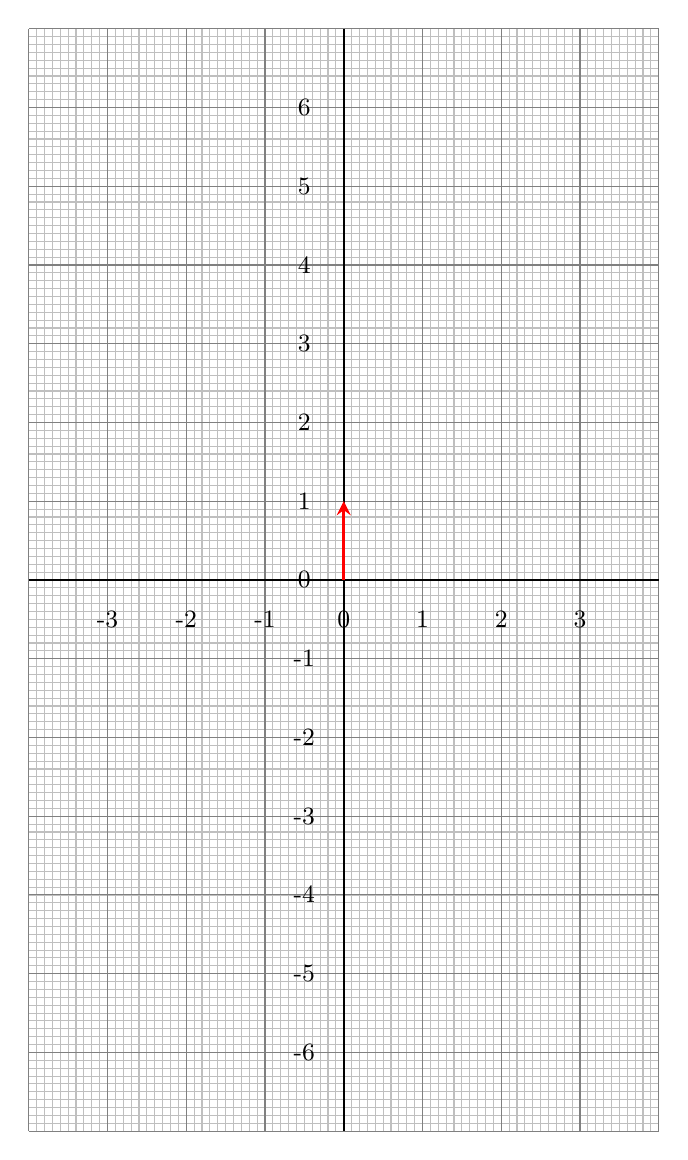
\begin{tikzpicture}
\draw[thin, step=0.1cm,color=lightgray] (-4,-7) grid (4,7);
\draw[thin, step=1cm,color=gray] (-4,-7) grid (4,7);
\draw[thick] (-4,0)--(4,0);
\draw[thick] (0,7)--(0,-7);
\foreach \x in {-3,...,3}{
  \node at (\x,-0.5)  {\small{\x}};
}
\foreach \y in {-6,...,6}{
  \node at (-0.5,\y)  {\small{\y}};
}
\draw [very thick, red, -stealth] (0,0)--(0,1);
\end{tikzpicture}
 \quad $answer$
\\
\end{tabular}
\newpage
Reflect the vector in the $x$-axis:
\newline
\newline
\begin{tabular}{p{9cm}p{9cm}}
a) 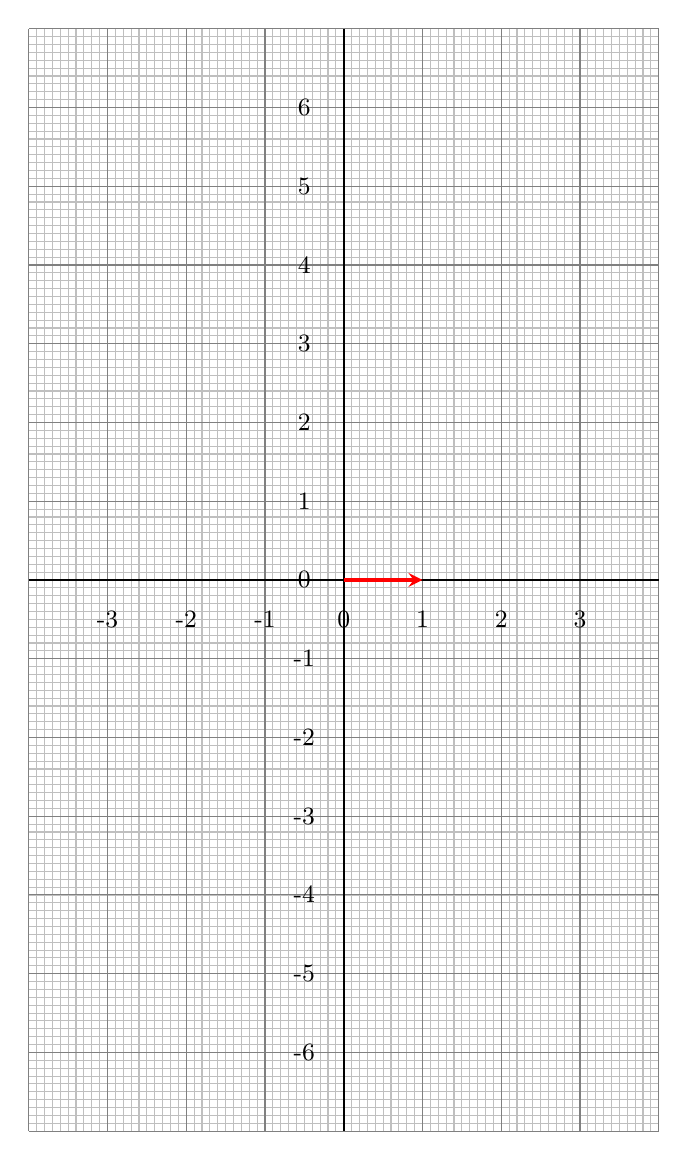
\begin{tikzpicture}
\draw[thin, step=0.1cm,color=lightgray] (-4,-7) grid (4,7);
\draw[thin, step=1cm,color=gray] (-4,-7) grid (4,7);
\draw[thick] (-4,0)--(4,0);
\draw[thick] (0,7)--(0,-7);
\foreach \x in {-3,...,3}{
  \node at (\x,-0.5)  {\small{\x}};
}
\foreach \y in {-6,...,6}{
  \node at (-0.5,\y)  {\small{\y}};
}
\draw [very thick, red, -stealth] (0,0)--(1,0);
\end{tikzpicture}
 \quad $answer$
&b) 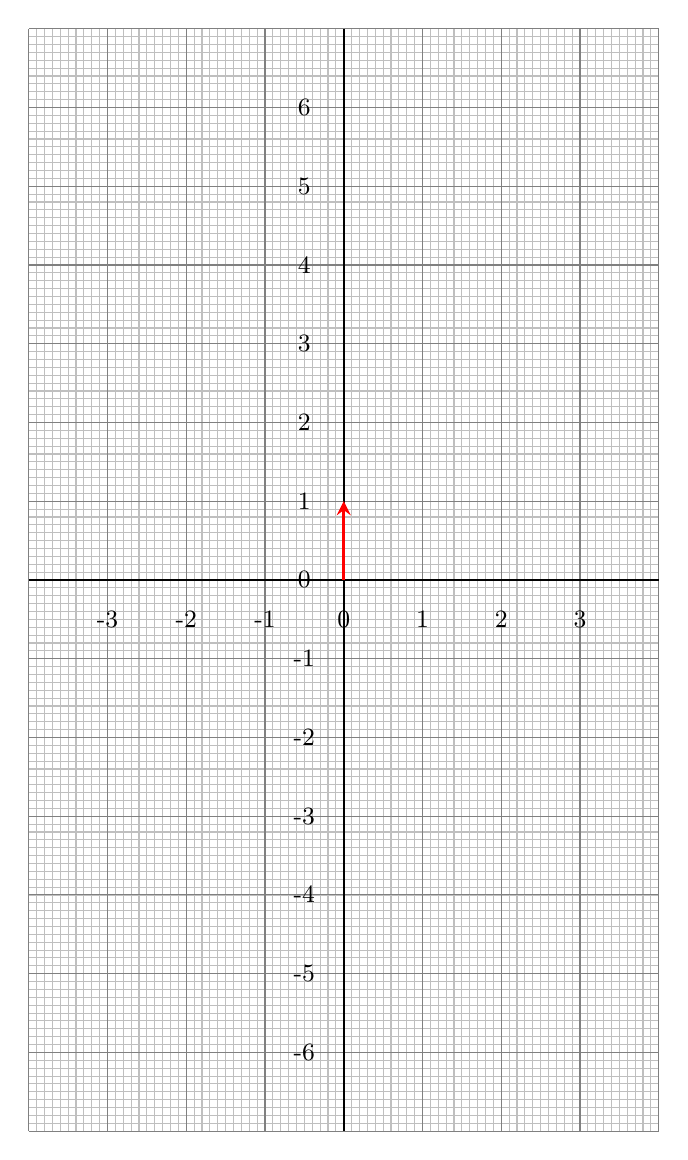
\begin{tikzpicture}
\draw[thin, step=0.1cm,color=lightgray] (-4,-7) grid (4,7);
\draw[thin, step=1cm,color=gray] (-4,-7) grid (4,7);
\draw[thick] (-4,0)--(4,0);
\draw[thick] (0,7)--(0,-7);
\foreach \x in {-3,...,3}{
  \node at (\x,-0.5)  {\small{\x}};
}
\foreach \y in {-6,...,6}{
  \node at (-0.5,\y)  {\small{\y}};
}
\draw [very thick, red, -stealth] (0,0)--(0,1);
\end{tikzpicture}
 \quad $answer$
\\
\end{tabular}
\newpage
Reflect the vector in the $y$-axis:
\newline
\newline
\begin{tabular}{p{9cm}p{9cm}}
a) 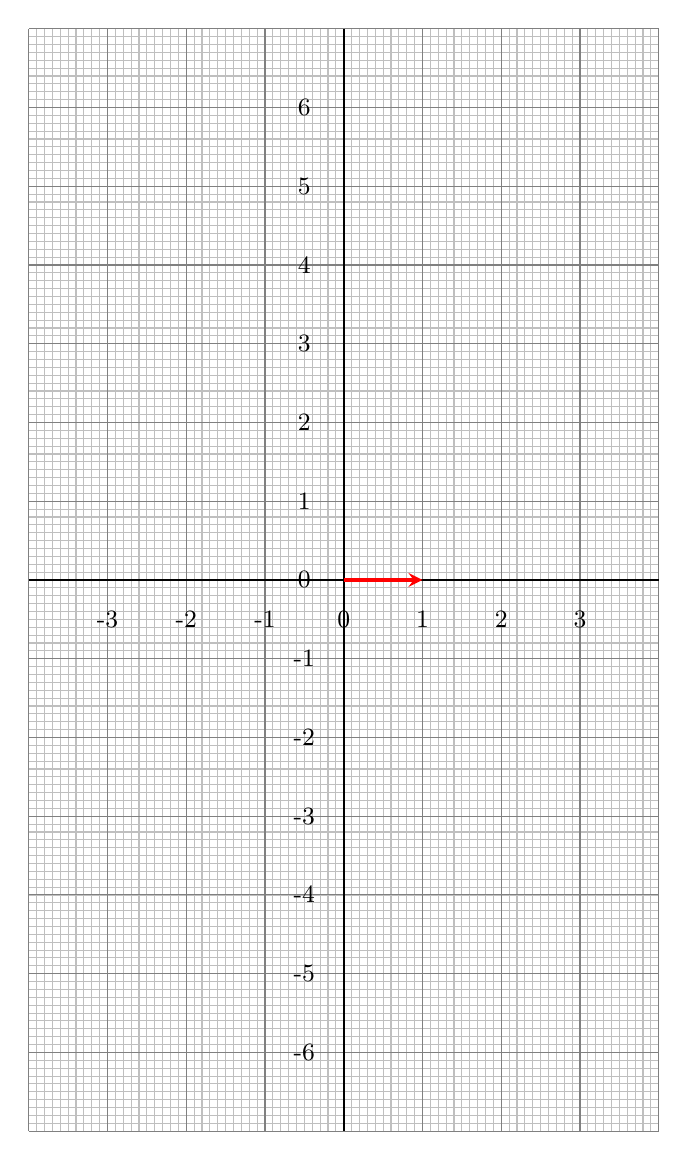
\begin{tikzpicture}
\draw[thin, step=0.1cm,color=lightgray] (-4,-7) grid (4,7);
\draw[thin, step=1cm,color=gray] (-4,-7) grid (4,7);
\draw[thick] (-4,0)--(4,0);
\draw[thick] (0,7)--(0,-7);
\foreach \x in {-3,...,3}{
  \node at (\x,-0.5)  {\small{\x}};
}
\foreach \y in {-6,...,6}{
  \node at (-0.5,\y)  {\small{\y}};
}
\draw [very thick, red, -stealth] (0,0)--(1,0);
\end{tikzpicture}
 \quad $answer$
&b) 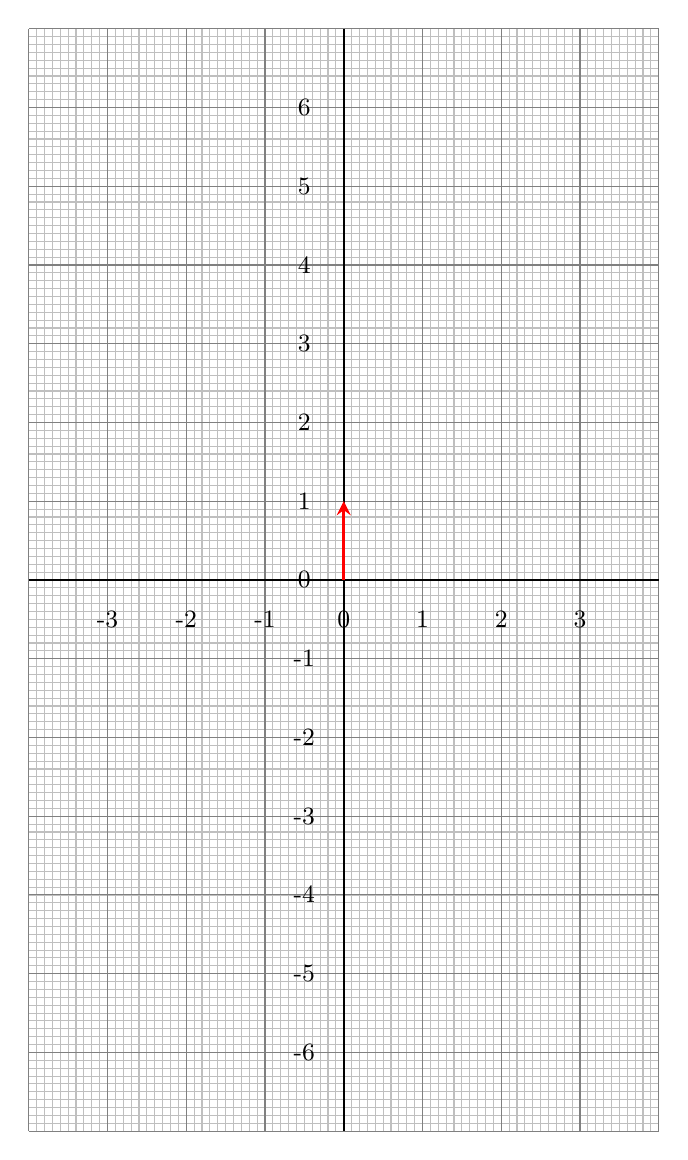
\begin{tikzpicture}
\draw[thin, step=0.1cm,color=lightgray] (-4,-7) grid (4,7);
\draw[thin, step=1cm,color=gray] (-4,-7) grid (4,7);
\draw[thick] (-4,0)--(4,0);
\draw[thick] (0,7)--(0,-7);
\foreach \x in {-3,...,3}{
  \node at (\x,-0.5)  {\small{\x}};
}
\foreach \y in {-6,...,6}{
  \node at (-0.5,\y)  {\small{\y}};
}
\draw [very thick, red, -stealth] (0,0)--(0,1);
\end{tikzpicture}
 \quad $answer$
\\
\end{tabular}
\newpage
Rotate the vector 90 degrees anti-clockwise:
\newline
\newline
\begin{tabular}{p{9cm}p{9cm}}
a) 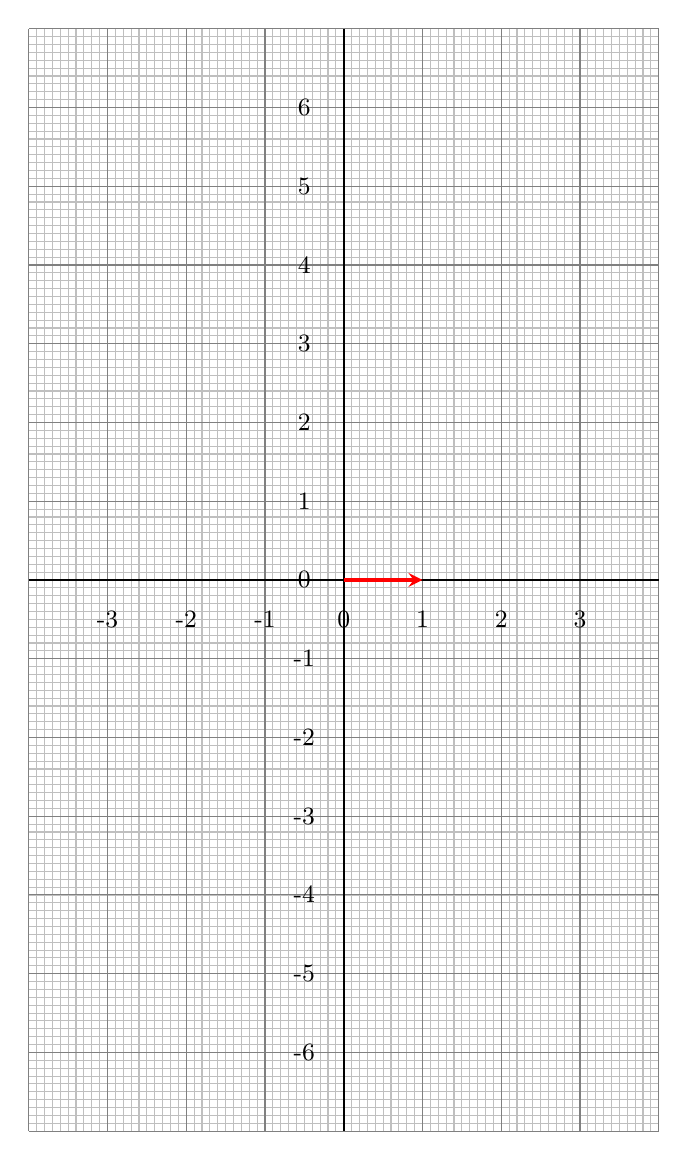
\begin{tikzpicture}
\draw[thin, step=0.1cm,color=lightgray] (-4,-7) grid (4,7);
\draw[thin, step=1cm,color=gray] (-4,-7) grid (4,7);
\draw[thick] (-4,0)--(4,0);
\draw[thick] (0,7)--(0,-7);
\foreach \x in {-3,...,3}{
  \node at (\x,-0.5)  {\small{\x}};
}
\foreach \y in {-6,...,6}{
  \node at (-0.5,\y)  {\small{\y}};
}
\draw [very thick, red, -stealth] (0,0)--(1,0);
\end{tikzpicture}
 \quad $answer$
&b) 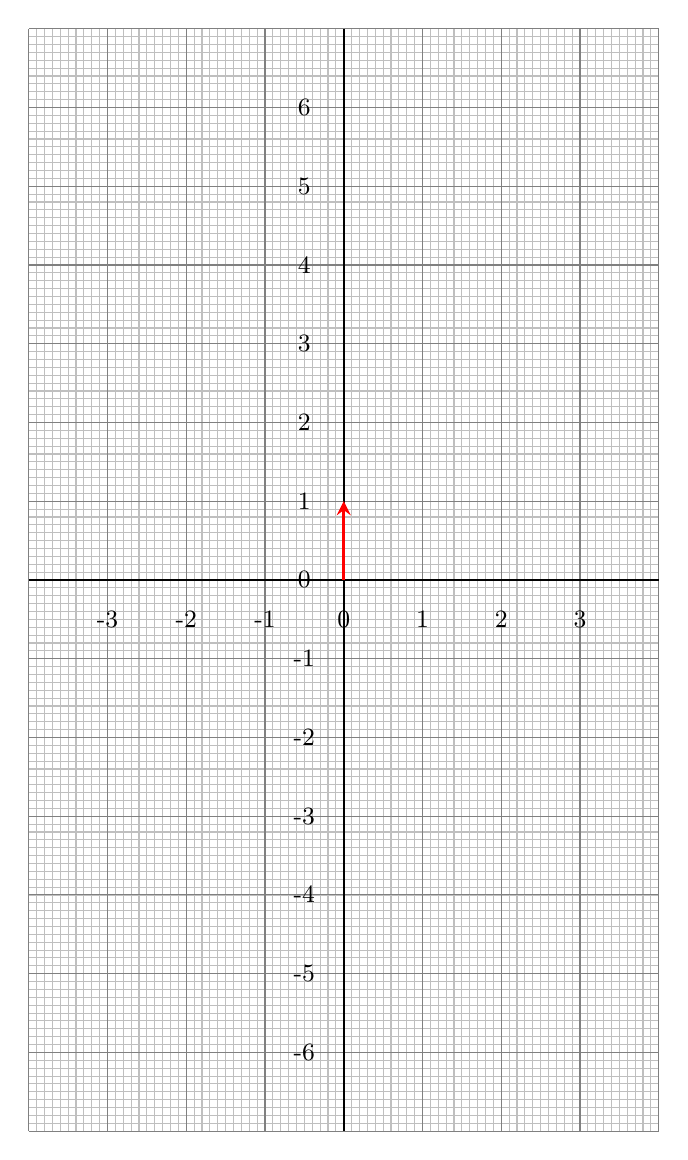
\begin{tikzpicture}
\draw[thin, step=0.1cm,color=lightgray] (-4,-7) grid (4,7);
\draw[thin, step=1cm,color=gray] (-4,-7) grid (4,7);
\draw[thick] (-4,0)--(4,0);
\draw[thick] (0,7)--(0,-7);
\foreach \x in {-3,...,3}{
  \node at (\x,-0.5)  {\small{\x}};
}
\foreach \y in {-6,...,6}{
  \node at (-0.5,\y)  {\small{\y}};
}
\draw [very thick, red, -stealth] (0,0)--(0,1);
\end{tikzpicture}
 \quad $answer$
\\
\end{tabular}
\newpage
Find a matrix which transforms the first vector into the second vector:
\newline
\newline
\begin{tabular}{p{9cm}p{9cm}}
a) $\begin{pmatrix}1\\0\end{pmatrix}, \begin{pmatrix}0\\1\end{pmatrix}$
 \quad $answer$
&b) $\begin{pmatrix}1\\0\end{pmatrix}, \begin{pmatrix}1\\0\end{pmatrix}$
 \quad $answer$
\\\\\\
\\\\\\

c) $\begin{pmatrix}1\\0\end{pmatrix}, \begin{pmatrix}-1\\0\end{pmatrix}$
 \quad $answer$
&d) $\begin{pmatrix}1\\0\end{pmatrix}, \begin{pmatrix}0\\-1\end{pmatrix}$
 \quad $answer$
\\\\\\
\\\\\\

e) $\begin{pmatrix}1\\0\end{pmatrix}, \begin{pmatrix}2\\0\end{pmatrix}$
 \quad $answer$
&f) $\begin{pmatrix}1\\0\end{pmatrix}, \begin{pmatrix}0\\-2\end{pmatrix}$
 \quad $answer$
\\\\\\
\end{tabular}
\newpage
Find a matrix which transforms the first vector into the second vector:
\newline
\newline
\begin{tabular}{p{9cm}p{9cm}}
a) $\begin{pmatrix}0\\1\end{pmatrix}, \begin{pmatrix}0\\1\end{pmatrix}$
 \quad $answer$
&b) $\begin{pmatrix}0\\1\end{pmatrix}, \begin{pmatrix}1\\0\end{pmatrix}$
 \quad $answer$
\\\\\\
\\\\\\

c) $\begin{pmatrix}0\\1\end{pmatrix}, \begin{pmatrix}-1\\0\end{pmatrix}$
 \quad $answer$
&d) $\begin{pmatrix}0\\1\end{pmatrix}, \begin{pmatrix}0\\-1\end{pmatrix}$
 \quad $answer$
\\\\\\
\\\\\\

e) $\begin{pmatrix}0\\1\end{pmatrix}, \begin{pmatrix}2\\0\end{pmatrix}$
 \quad $answer$
&f) $\begin{pmatrix}0\\1\end{pmatrix}, \begin{pmatrix}0\\-2\end{pmatrix}$
 \quad $answer$
\\\\\\

\end{tabular}
\end{document}
